\subsection*{Defining data elements}

\begin{figure*}
\ifthenelse{\boolean{plosone}}{
  \begin{adjustwidth}{-2.25in}{0in}
}{}
 % Comment out/remove adjustwidth environment i

\begin{tabular}{p{0.5\textwidth}p{0.5\textwidth}}
{\sf \large A} & {\sf \large B}
\\
\vspace{0pt}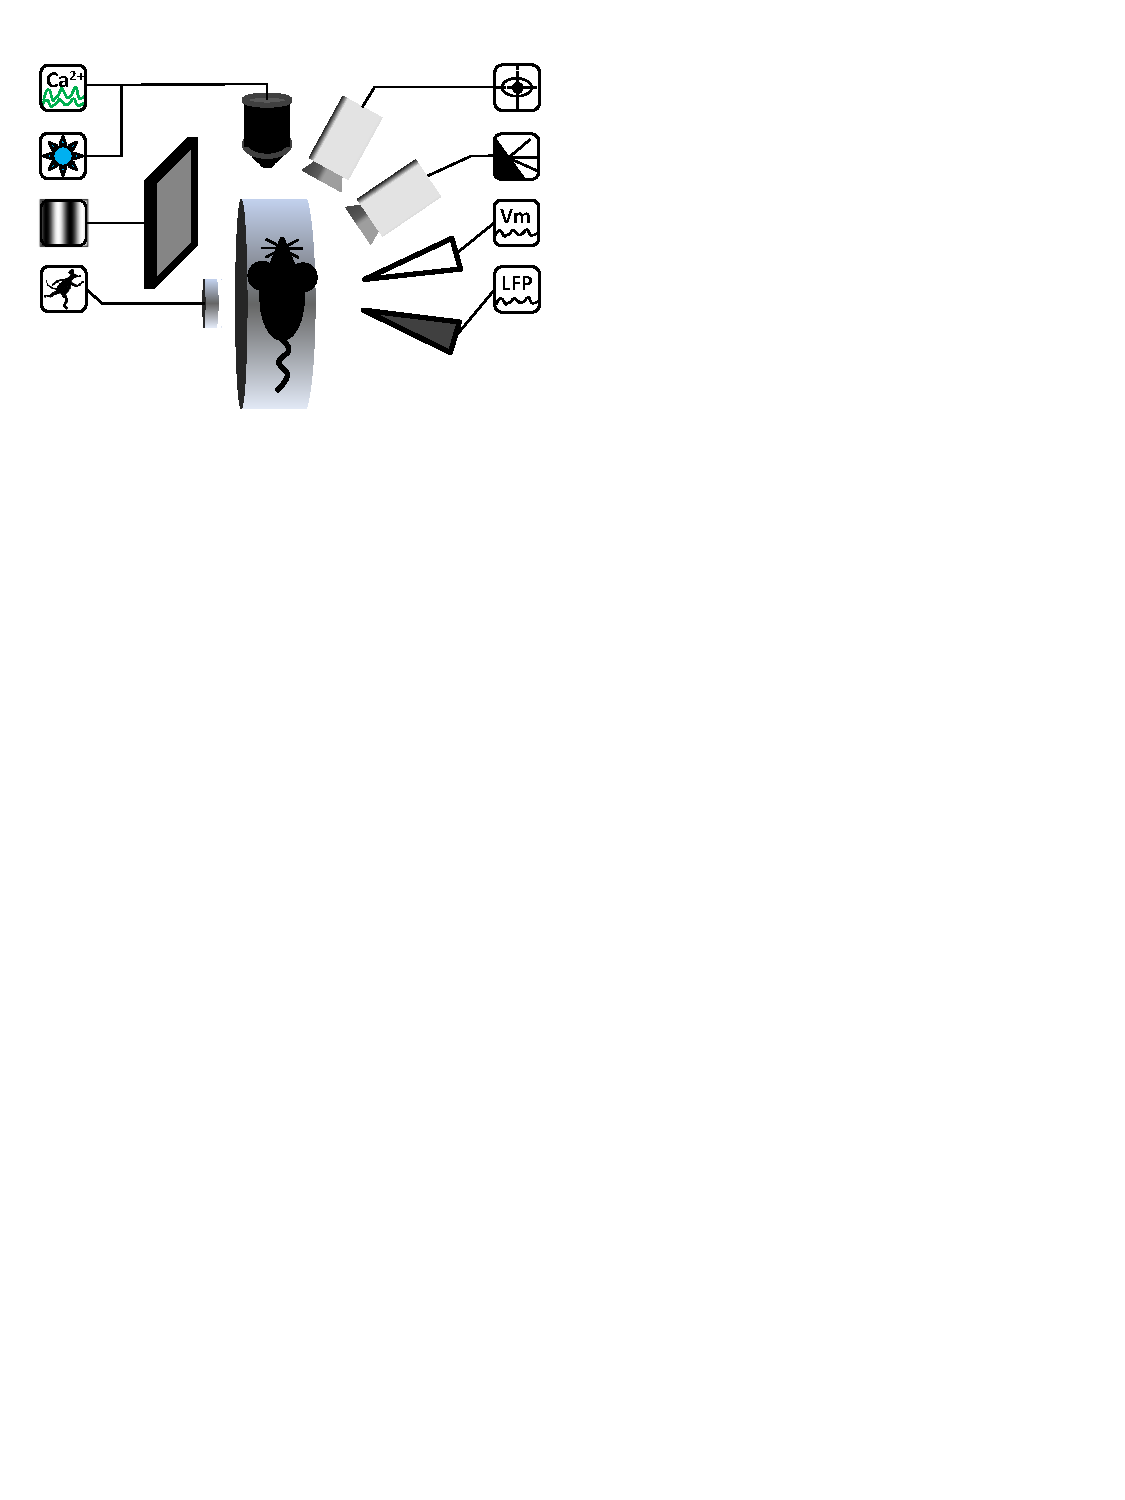
\includegraphics{./figures/experiment.pdf} &
\vspace{0pt}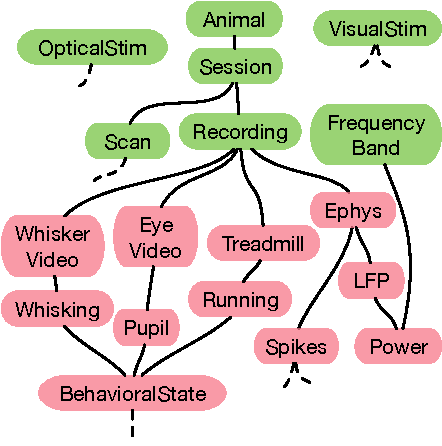
\includegraphics{./figures/schema.pdf}
\\
\end{tabular}

{\sf \large C}
\vspace{6pt}

\inputminted[frame=single,linenos=true]{python}{Session.py}

\vspace{6pt}
{\sf \large D}
\vspace{6pt}

\csvreader[
table head = \hline\bf animal & \bf session & \bf user & \bf session\_date & \bf session\_folder & \bf notes & \bf timestamp\\\hline,
before table=\rowcolors{1}{white}{Beige},
table foot = \hline,
head to column names,
tabular=|cc|lllll|
]{session.csv}{}%
{\tt\animal & \tt\session & \tt\user & \tt\date & \tt\folder & \tt\notes & \tt\ts}
\caption{
{\bf An example experiment and its DataJoint schema.}
{\sf A.}  
A neuroscience experiment with multiple stimulation and acquisition modalities (counterclockwise from top left corner): fluorescence imaging of calcium signals (Ca$^{2+}$), light stimulation of optogenetic probes, visual stimulus, treadmill motion recording, local-field potential recording (LFP), whole-cell patch membrane potential recording (V\textsubscript{m}), video of whisker movements, video of eye movements.
{\sf B.}  The entity relationship diagram (ERD) of a DataJoint schema comprising base relations storing externally entered data (green) and automatically populated data (red).
{\sf C.}  
The Python class for the base relation \mintinline{python}{Session} specifying the relation's heading. 
A dependency on \mintinline{python}{Animal} is indicated with the arrow {\tt-\textgreater}.  
An additional primary key attribute, {\tt session}, enables multiple sessions per animal. 
Dependent attributes are separated from primary key attributes by {\tt---}.   
Each attribute has a name, an optional default value, a datatype, and an optional comment.
{\sf D.}  
Example contents of \mintinline{python}{Session}.
The vertical divider separates the primary key attributes `{\tt animal}' and `{\tt session}` from the dependent attributes.
} 
\label{schema}
\ifthenelse{\boolean{plosone}}{\end{adjustwidth}}{}
\end{figure*}
 

Consider a particular real-world neuroscience study comprising a series of experiments that involve simultaneous \emph{in vivo} recordings of several types of physiological signals (whole-cell membrane potential or V\textsubscript{m}, local-field potentials or LFP, and calcium fluorescence signals), stimuli (visual display and optogenetic stimulation of targeted neuronal populations), and behaviors (locomotion, whisking, eye movements) \cite{reimer_pupil_2014}. 
Figure \ref{schema}\,A illustrates such an experiment.

To work with data from such studies, DataJoint users create a \emph{schema} (or several schemas) comprising a collection of \emph{base relations} to represent the various elements of the experiments (Fig.\ \ref{schema}\,B).
Relations are DataJoint's basic data representation and can be thought of as simple tables with a \emph{heading} and a \emph{body}.
The heading specifies attribute names and datatypes. 
The body comprises a set of \emph{tuples} of attribute values. 
Base relations are stored in the database whereas \emph{derived relations} may be constructed from base relations for data queries.
For detailed definitions of the Relational Data Model, see Table \ref{glossary}.

\ifthenelse{\boolean{plosone}}{
  \begin{figure*}
  \begin{adjustwidth}{-1.in}{0in} % Comment out/remove adjustwidth environment i
}{
  \begin{table*}
}

\begin{boxedminipage}{\textwidth}
\section*{Relational Data Model}
\begin{description}
\setlength\itemsep{6pt}
\item[Relation] 
All data are represented as \emph{relations}.  A relation can be visualized as a table or a shreadsheet.  
It consists of a \emph{heading} with attribute names and datatypes and a \emph{body} comprising a set of \emph{tuples} with values for each attribute.

\begin{center}
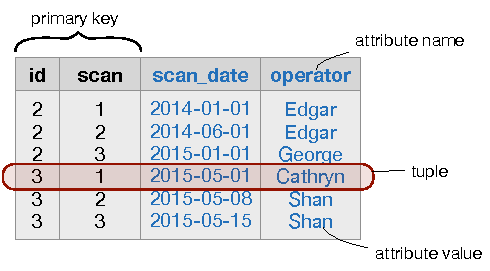
\includegraphics{./figures/relation.pdf}
\end{center}

We distinguish between \emph{base relations} and \emph{derived relations}.  
A base relation has a dedicated class in MATLAB or Python and represents data stored directly in the database.
Derived relations are formed from other relations by using relational operators (See Table \ref{algebra}).
To create a new base relation, users create a new MATLAB or Python class subclassing from the DataJoint Relation class and define the relation's heading. 
After that, users interact with the data by invoking these relation classes.

\item[Schema] A schema is a named collection of related base relations. 
A single project may store data across multiple schemas. Conversely, many schemas can be used for data shared by multiple projects.

\item[Query] Queries retrieve the data represented by a relation into the MATLAB or Python workspace.

\item[Primary key] Every relation has a primary key: a subset of its of attributes that uniquely identify each of its tuples. 
Two tuples with the same values of the primary key attributes cannot coexist in the same relation.
The remaining attributes in the relation are called dependent attributes. 
When one relation includes some attributes that also belong to the primary key of another relation, they determine how tuples are grouped and related between the two relations.

\item[Dependencies]
Base relations may form dependencies by referencing one another. 
Every tuple in a dependent relation must have a matching tuple in the relations references by the dependency. 
Dependencies may cross schema boundaries.

\item[ERD]
The entity relationship diagram or ERD is a graphical representation of base relations and their dependencies.
Fig.\ \ref{schema}\,B depicts the ERD for a particular neuroscience experiment. 
\end{description}
\end{boxedminipage}
\caption{Key concepts of the relational data model as used in DataJoint.}
\label{glossary}

\ifthenelse{\boolean{plosone}}{
  \end{adjustwidth}
  \end{figure*}
}{
  \end{table*}
}


A base relation is created in the form of a class in MATLAB or Python (Fig.\ \ref{schema}\,C) that defines the relation's heading.
The heading definition comprises a description of the relation, dependencies on other base relations, and a set of \emph{attributes}. 
Each attribute has a name, an optional default value, a datatype, and an optional description.
Attributes that comprise the \emph{primary key} of the relation are separated from the remaining attributes by the divider {\tt---}.

DataJoint provides all the functionality for accessing and manipulating data through the base relation classes. 

